\documentclass[a4paper,14pt]{extarticle} \usepackage[utf8]{inputenc}
\usepackage[T1]{fontenc}
\usepackage[margin=2.5cm]{geometry}

% Fonte Caladea se existir, senão lmodern
\IfFileExists{caladea.sty}{
  \usepackage{caladea}
}{
  \usepackage{lmodern} }
\usepackage{ragged2e}
\usepackage{graphicx}
\usepackage[portuguese]{babel}
\usepackage{wrapfig}
\usepackage{hyperref}
\usepackage{fancyhdr}
\usepackage{xcolor}
\usepackage{rotating}
\usepackage{titlesec}
\usepackage{epigraph}
\usepackage{dirtytalk}
\usepackage{indentfirst} % Indenta o primeiro parágrafo após seções

% Ajuste do recuo de parágrafo
\setlength{\parindent}{1.5em}

% Adjust headheight to remove LaTeX warning
\setlength{\headheight}{17.54163pt}

% Centralizar títulos
\titleformat{\section}
  {\normalfont\centering\bfseries\Large}{}{1em}{}

\titleformat{\subsection}
  {\normalfont\centering\bfseries\large}{}{1em}{}

\titleformat{\subsubsection}
  {\normalfont\centering\bfseries}{}{1em}{}

% -------------- Símbolos de Versículo e Resposta --------------
% Definição do símbolo (a “barrinha” inclinada)
\makeatletter
\newcommand{\vers@resp@sym}{%
  \raisebox{0.2ex}{\rotatebox[origin=c]{-20}{$\m@th\rceil$}}%
}
% macro interna que sobrepõe a barrinha e a letra V ou R
\newcommand{\vers@resp}[2]{%
  {\ooalign{%
     \hidewidth\kern#1\vers@resp@sym\hidewidth\cr
     #2\cr
  }}%
}
% comandos públicos \versicle e \response
\DeclareRobustCommand{\versicle}{\vers@resp{-0.1em}{V}}
\DeclareRobustCommand{\response}{\vers@resp{0pt}{R}}
\makeatother
% ^------------- Símbolos de Versículo e Resposta -------------^

% Rodapé com imagem e página
\pagestyle{fancy}
% ---- Cabeçalho ------------
\fancyhf[C]{}
% ----- Rodapé --------------
\fancyfoot[C]{%
  
\includegraphics[scale=0.2]{assets/cross.png}\quad
  \textit{\textit{Critos, tende piedade de nós.}}\quad
  \thepage
}

\usepackage{pdfpages}
\begin{document}
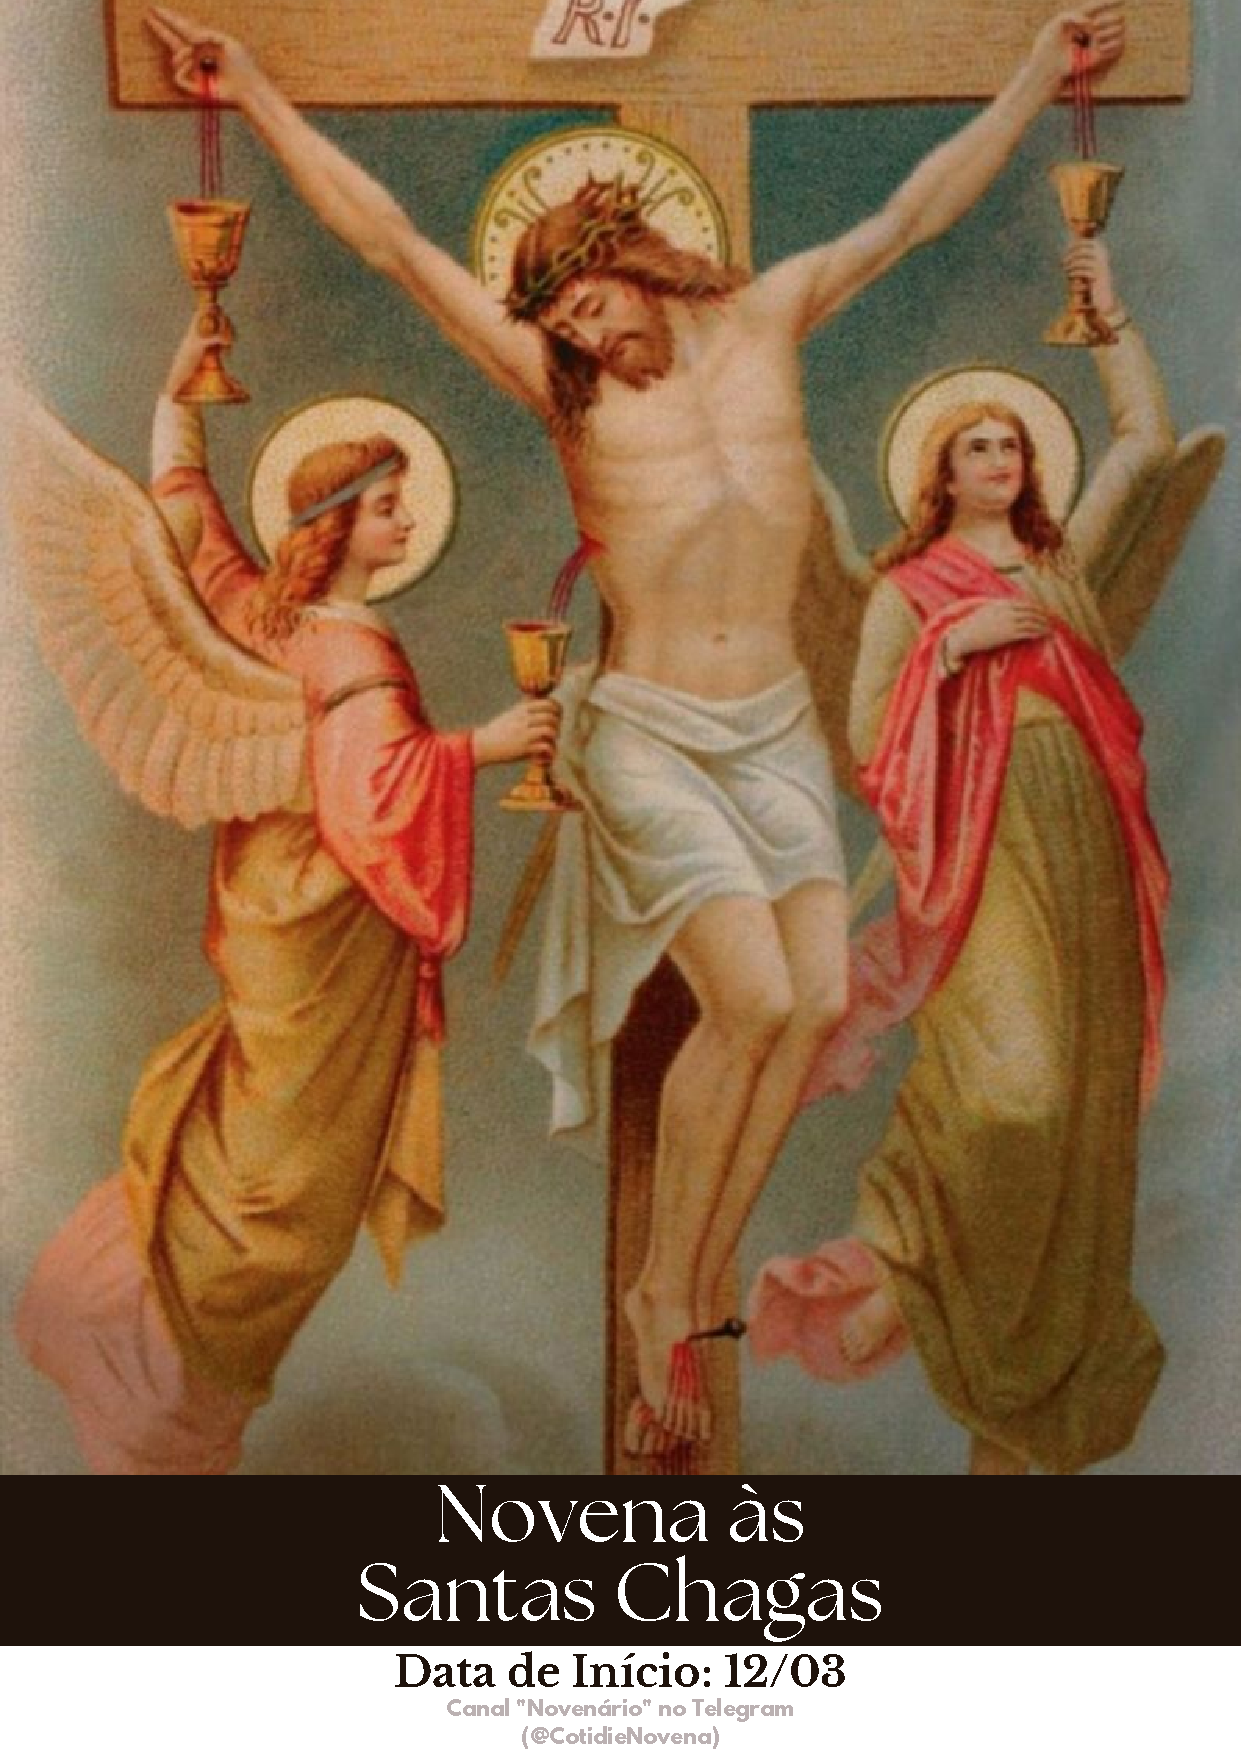
\includepdf[pages=1]{Capa Santas Chagas.pdf}

\begin{center}
	{\huge Novena de Santas Chagas}
\end{center}



\noindent\rule{\textwidth}{0.4pt}

\tableofcontents

\thispagestyle{empty}


% --- Origem ---
\newpage

\section{História}

Há devoções tão antigas como o Calvário e que tiveram pontos altos na vida e na história da Igreja. Entre estas está a devoção das Santas Chagas.

Parece ser da vontade de Deus reavivar tal devoção, como meio de santificação pessoal e reparação pelos pecadores. Perante tanta maldade e desordem, desprezo pelo divino e indiferença pela ofensa ao Criador, só a reparação pode salvar o mundo. Daí a necessidade de almas reparadoras. E a devoção das Santas Chagas é eminentemente reparadora.

Santo Agostinho, São João Crisóstomo, São Bernardo, São Boaventura, São Tomás de Aquino e São Francisco de Assis fizeram desta devoção objeto especial do seu zelo apostólico.

Em seu livro de 1761, A Paixão e a Morte de Jesus Cristo, Santo Afonso Maria de Ligorio, fundador dos Padres Redentoristas, listou, entre vários exercícios piedosos, o Terço das Cinco Chagas de Jesus Crucificado. O Rosário das Santas Chagas foi introduzido pela primeira vez no início do século 20 pela Venerável Irmã Maria Marta Chambon, religiosa católica romana leiga do Mosteiro da Ordem de Visitação em Chambéry, França.


\subsection{As Santas chagas}

O Senhor, ao manifestar-Se à Irmã Maria Marta Chambon, do Mosteiro da Visitação de Santa Maria Chambery, falecida em odor de santidade em 21 de Março de 1909, encarregou-a de invocar constantemente as Suas Chagas e de avivar esta devoção no mundo. Para este fim, revelou-lhe com palavras vivas os tesouros que encerram essas feridas abertas na Sua Carne imaculada.
Deveis repetir com freqüência, junto aos doentes esta aspiração: "MEU JESUS, PERDÃO E MISERICÓRDIA, PELOS MÉRITOS DE VOSSAS SANTAS CHAGAS." Esta oração aliviará a alma e o corpo. Muitas pessoas experimentarão a eficácia destas aspirações.
O pecador que disser a oração seguinte, alcançará perdão: \say{PAI ETERNO, EU VOS OFEREÇO AS CHAGAS DE NOSSO SENHOR JESUS CRISTO, PARA CURAR AS DE NOSSAS ALMAS.}
% --- Orações Diárias ---
\newpage

\vfill

\section{Orações}
\subsection{Oração de Todos os Dias}\label{sub:inicial} % (fold)

{
	\noindent
	† Por Suas Santas Chagas\\
	† Suas chagas Gloriosas\\
	† O Cristo Senhor me proteja e me guarde\\
}

Senhor Jesus, foste elevado na Cruz para que por Vossas Santas Chagas, sejam curadas as de nossas almas. Eu Vos louvo e agradeço pelo Vosso ato redentor. Carregaste em Vosso próprio corpo os meus pecados e de toda a humanidade. Nas Vossas Santas Chagas coloco minhas intenções. Minhas preocupações, ansiedades e angustias. Minhas enfermidades físicas e psíquicas. Meus sofrimentos, dores, alegrias e necessidades. Em vossas Santas Chagas Senhor coloco minha família. Envolvei Senhor a mim e meus familiares protegendo-nos do mal.

\textit{(instante de silencio)}

Senhor, ao mostrar Vossas Santas Chagas Gloriosas a Tomé e o mandando tocar em Vosso lado aberto, o curaste da incredulidade. Eu Vos peço, Senhor, permita-me refugiar em Vossas Santas Chagas e por mérito desses sinais de Vosso amor curai a minha falta de fé. Ó Jesus, pelos méritos de Vossa Paixão, Morte e Ressurreição, dai-me a graça de viver os frutos da nossa redenção.
Amém.

\vfill

\begin{center}
	\subsection*{Fontes:}
	Adaptado de: {\color{blue} \underline{\href{https://pocketterco.com.br/terco/novena-das-santas-chagas}{Pocket Terço}}}

\end{center}


\end{document}
